\documentclass[conference]{IEEEtran}
\IEEEoverridecommandlockouts
% The preceding line is only needed to identify funding in the first footnote. If that is unneeded, please comment it out.
\usepackage{cite}
\usepackage{amsmath,amssymb,amsfonts}
\usepackage{algorithmic}
\usepackage{graphicx}
\usepackage{textcomp}
\usepackage{xcolor}
\usepackage[hidelinks]{hyperref} % add links, but don't highlight them
\usepackage{cleveref} % better references
\usepackage{float}
\usepackage{enumitem}
\usepackage{esvect}
\usepackage{pgfplots}
\pgfplotsset{compat=newest}
%\usepackage{flushend} % balance last page
\usepackage{soul}

\usepackage{tabu}
\usepackage{booktabs}
\usepackage{tikz}

\usepackage{enumitem}
\usepackage{comment}

%
% ---- notes in text ---
%
\usepackage{xargs}                      
\usepackage[pdftex,dvipsnames]{xcolor}  

\usepackage[colorinlistoftodos,prependcaption]{todonotes} % ,textsize=tiny
\newcommandx{\unsure}[2][1=]{\todo[linecolor=blue,backgroundcolor=blue!25,bordercolor=blue,#1]{#2}}
\newcommandx{\change}[2][1=]{\todo[linecolor=red,backgroundcolor=red!25,bordercolor=red,#1]{#2}}
\newcommandx{\info}[2][1=]{\todo[linecolor=green,backgroundcolor=green!25,bordercolor=green,#1]{#2}}
\newcommandx{\improvement}[2][1=]{\todo[linecolor=Plum,backgroundcolor=Plum!25,bordercolor=Plum,#1]{#2}}
\newcommandx{\thiswillnotshow}[2][1=]{\todo[disable,#1]{#2}}

\usepackage[colorinlistoftodos]{todonotes}


\def\BibTeX{{\rm B\kern-.05em{\sc i\kern-.025em b}\kern-.08em
    T\kern-.1667em\lower.7ex\hbox{E}\kern-.125emX}}
\begin{document}

    %\title{ZkServe - Verifiable Data Services for Decentralized Sharing and Trading}
	\title{Policy Compliance in Local Energy Markets}

	%\author{\IEEEauthorblockN{1\textsuperscript{st} Jonathan Heiss}
	\author{\IEEEauthorblockN{Alvaro Alonso Domenech, Stefan Krakan}
		\IEEEauthorblockA{\textit{Information System Engineering } \\
			\textit{Technische Universität Berlin}\\
			Berlin, Germany \\
	{\{aa\}}@ise.tu-berlin.de, stefan@krakan.de}
	}

	 %\newcommand\copyrighttext{%
	 %\footnotesize  Pre-Print Version, \textcopyright 2019 IEEE. Personal use of this material is permitted.
	 %Permission from IEEE must be obtained for all other uses, in any current or future
	 %media, including reprinting/republishing this material for advertising or promotional
	 %purposes, creating new collective works, for resale or redistribution to servers or
	 %lists, or reuse of any copyrighted component of this work in other works.
	%DOI: \href{<http://tex.stackexchange.com>}{<DOI No.>}
	 %}
   %\newcommand\copyrightnotice{%
   %\begin{tikzpicture}[remember picture,overlay]
   %\node[anchor=south,yshift=10pt] at (current page.south) {\fbox{\parbox{\dimexpr\textwidth-\fboxsep-\fboxrule\relax}{\copyrighttext}}};
   %\end{tikzpicture}%
   %}

	\maketitle
	%\copyrightnotice

	\begin{abstract}
    \todo[inline]{Do in the end}
	\end{abstract}

	\begin{IEEEkeywords}
		Blockchain, GDPR-compliance, Consent Violation Detection, Incentive Mechanisms
	\end{IEEEkeywords}

	\section{Introduction}
	\label{sec:introduction}
	
\todo[inline]{shorten / refine}

In recent years climate change has become one of the most important issues for humanity. 
To target climate change effectively, strategies need to be implemented in order to reduce carbon emissions and transition towards sustainable energy sources. 

Effective climate governance requires a polycentric approach, by increasing the role of non-state actor and employing diverse actions by multiple actors at various levels and industries \cite{Huitema2010GoverningCC}. Furthermore, local actions become important in climate governance, as small-scale initiatives can often be more effective and adaptable to specific circumstances. 
However, existing implementations of local policies and programs intended to govern  this global common are inefficient and highlight institutional weaknesses \cite{brazilCommons}. Not only is it challenging to implement effective monitoring of the transition to renewable energy sources but also the potential to infringe upon personal freedoms and privacy is a concern \cite{molina2010private}. Yet, this data collection is necesarry in order to applly proper incentives and punishment and  to assess the impact and effectiveness of climate policies and environmental initiatives. \info[inline]{add resources that underline the importance of measuring data in order to apply proper punishments and rewards} 

In this regard, building systems that empower local communitites and incentivise them to support the achievment of societal objectives enables effective polycentric climate governance. While each household’s energy consumption might seem minor in isolation, collectively, they form a substantial part of the overall energy footprint. by implementing compliance verification systems that allows for policy verification in local energy markets, the transisition towards renewables energy sources of communities can be tackeld more effectively.  This provides a tangible way to assess the impact and effectiveness of climate policies and environmental initiatives. Furthermore it enables the tracking of progress and provision of incentives, while also holding households accountable for their energy consumption and environmental impact.

This issue can be further complicated by the global increase in state monitoring and data collection in recent years, as Eck et al. \cite{surveill} note. They caution that such practices could pose threats to privacy rights and democratic norms, which emphasises the need for systems that can fulfil societal goals without compromising these fundamental principles.


Therefore, building systems that achieve a balance between compliance and privacy might be a key factor in gaining public trust and support for climate action policies. Furthermore, such systems can reduce state intervention and monitoring, while simultaneously empowering communities by encouraging shared responsibilities and collective-driven initiatives. 

This paper introduces a system that allows effective and verifiable compliance checks at a collective level, while still protecting individual privacy, as can be seen in Figure 1.1. In order to accomplish this, the nesting of Zero-Knowledge Proofs (ZKP) will be applied

We make the following three individual contributions:
\begin{itemize}
    \item
    \item
    \item
\end{itemize}

\todo[inline]{Paper outline here}


	\section{Background}
	\label{sec:preliminaries}
	

\subsection{Climate Change in CS World}
Climate change is targeted from computer science two-fold \cite{cs_cc}: by mitigating the direct negative impact of computers on the environment through reduction of energy consumption and associated socio-economic costs and by enhancing existing processes to improve their efficiency. As this paper focuses on the latter, we wont discuss the mitigation of its negative impact further. 

In mitigation and adaptation strategies for existing systems, Machine Learning (ML) \cite{MachineLearning} and Artificial Intelligence (AI) \cite{AI_CC} could be utilised, such as enhancing energy systems, optimizing transportation or aiding urban planning. However, their net impact on carbon emissions remains ambiguous due to the increased demand for hardware and energy \cite{AI_CC_2}. 




\subsection{Compliance}

\subsection{ZKPs}

	\section{Related Work}
	\label{sec:relatedWork}
	We position our contributions within related work on 


Although studies specifically focusing on privacy-preserving methods for policy compliance in local renewable energy markets are scarce, there is a considerable body of research dedicated to the broader areas of privacy-preserving data aggregation and smart metering. This highlights a notable gap in research that specifically connects these areas to energy compliance. This section will focus on few selected studies to illustrate the spectrum of approaches in the field.

We will start by exploring more general privacy-preserving data aggregation protocols beyond the context of smart metering and then delve into protocols specifically tailored for smart metering, also in connection with ZKPs. Following this work regarding ZoKrates in the context of privacy-preserving data aggregation and its applicability to smart meter data will be discussed. Lastly, we will examine the a gap in existing literature concerning the topic of nesting. However, we can explore some practical work regarding the closely related concept of recursion in relation to ZKPs.

\section{Methods in Privacy-Preserving Data Aggregation (PDA)}

As previously introduced, the aim this thesis is to develop a system that allows effective and verifiable compliance checks at a collective level, while still protecting individual privacy. Therefore, it is essential to privately aggregate data. This objective parallels the goal of PDA from existing literature. PDA protocols have been introduced to aggregate data from multiple sources and calculate statistics on sensitive data without infringing upon privacy \cite{PDA}. Even though not all the works discussed in this chapter are explicitly labelled as PDA, they are categorised as PDA, as they align with the definition from above. Bearing this in mind, this section discusses alternative approaches to PDA that do not necessarily rely on ZKPs, which highlights different potential  technologies for achieving similar objectives.


\subsection{Hypergraph-Based PDA}
Dekker et al. \cite{PDA} propose a PDA protocol, which employs a hypergraph-based detection algorithm, that probabilistically detects out-of-range user values without disclosing them to the aggregator. This protocol is suitable for aggregators working with resource-constrained users, as the hypergraph structure allows the aggregator to quickly pinpoint malicious users by examining the intersection of groups that deviate from the range. Furthermore, this protocol enables advanced algorithms like principal component analysis and decision tree classifications. However, the detection mechanism is inherently probabilistic, meaning it operates based on likelihood rather than absolute certainty. While the protocol offers strong privacy assurances, there exists a limit of colluding users beyond which privacy can be compromised.

\subsubsection{Dekker's et al. \cite{PDA} Remarks on ZKPs for PDA\label{sec:malicious}}

They note that a shortcoming of much previous research is the assumption of \textit{honest-but-curious} participants for PDA protocols, a model where parties are expected to follow the protocol but may attempt to learn additional information. Dekker et al. acknowledge the potential to overcome this limitation by transitioning to a \textit{malicious model}, which can be achieved through the implementation of ZKPs. However, as traditional ZKP approaches rely on a trusted setup, such as zk-SNARKs, and the computationally intensive proof generation, render them less attractive for trustless or resource constrained scenarios. 

\subsection{Utilising Homomorphic Encryptions for Smart Meter Data\label{sec:homo}}

Alternatively, Mohamadali et al. \cite{nhp3} introduce a protocol for data aggregation in smart grids, that employs Paillier encryption. Their protocol has various features including batch verification, fault tolerance and support for multi-category data aggregation. These features enable more detailed insights into energy demand or load. While this protocol is efficient in terms of computational resources and secure under malicious models, it has a single point of failure, due to a centralised trusted authority that manages the whole system.

Similarly, Zhang et al. \cite{homo1} utilise Paillier encryption for both temporal and spatial data aggregation in smart grids, to provide utility companies with the necessary information for billing and grid management. In this context, "temporal aggregation" refers to combining data points over time and "spatial aggregation" across different locations. While it is secure under malicious models as well, they acknowledge in their security analysis that their system depends on certain technical conditions to ensure privacy, such as requiring non-symmetric data matrices and multi-element user sets.

While there are several more studies that leverage homomorphic encryption for data aggregation in smart grids, this section briefly introduced those two studies, to illustrate this approach. However in summary, while these approaches allow for privacy-preserving computations on encrypted data, they  may not fully address the more complex, multi-layered computation and verification processes that will be introduced in this thesis.

\subsection{Utilising ZKPs for Energy Billing}

ZKPs have been implemented to verify energy usage for billing purposes in smart grids, while ensuring that the actual consumption data stays confidential.

Rial et al. \cite{rial2011privacy} propose a system where electricity customers can compute non-interactive ZKPs on personal devices, that verify whether their consumption falls in certain billing tariffs without disclosing any meter data. The system supports a variety of tariffs, including time-of-use tariffs. They demonstrate that a single computer could verify billing proofs from a three week period of 27 million households in 12 days, even in their slowest unoptimised version. However their performance evaluation considers only proof size along with proof and verification time, ignoring the complexities involved in setting up the proof system.

In a separate study, Jawurek et al.  \cite{jawurek2011plug} introduce a plug-in privacy component, such as a router, which generates ZKPs based on Pedersen commitments. The proof confirms the consumers time-of-use tariff without disclosing any consumption data. Unlike the study of Rial et al. \cite{rial2011privacy} this study is limited to a single tariff system. 

More studies integrating ZKPs with smart metering will be discussed in later sections of this chapter where they are more contextually relevant.

\subsection{Blockchains and Ledgers in PDA}

Studies employing blockchains for PDA often combine these technologies with privacy-preserving methods, such as Bloom filters, homomorphic encryption, or ZKPs. This section will introduce some studies to provide an overview of the field.

Mouris and Tsoutsos’ "Masquerade" protocol \cite{masq} offers a lightweight general-purpose protocol for verifiable data aggregation, optimised for computing aggregated statistics, such as histograms and averages. They are utilising Paillier encryption to encrypt private data, ZKPs to verify the correctness of the computations and the Fiat-Shamir heuristic to convert interactive ZKPs to non-interactive ones. Furthermore the protocol is adaptable enough to support smartphone clients in dynamic user environments. Despite its strengths, the reliance on a central entity managing the ledger introduces a potential single point of vulnerability and their protocol has not been peer-reviewed.

The study by Mahmoud et al. \cite{mahmoud2019secure} contributes to the field PDA through its blockchain-based approach for Water Distribution Systems (WDS). It presents a method for aggregating smart meter data while providing user anonymity, applying blockchain to protect against data tampering and Bloom filters for identity verification. In doing so, the operational process becomes more transparent, as water quality and quantity or collected data, such as pipeline pressure, become verifiable. However the study acknowledges that their implementation faces immense challenges, because their blockchain's consensus algorithm relies on mining, which necessitates special mining nodes, that consume excessive energy and may not be suitable for most sensors, such as smart meters or hydraulic sensors.

Similarly, Guan et al. \cite{block2} encounter comparable challenges with their mining nodes to run blockchains for PDA in smart grids. Their approach involves dividing users into groups, each with its own blockchain that records data. Similarly again, they utilise bloom filters to authenticate users. This system faces challenges in balancing privacy, computational overhead and real-time data processing as well.

Homomorphic encryption is a popular choice, as multiple other studies also combine it with  blockchain. For example, Fan et al. \cite{block_fan} utilise this approach along with leader election algorithms and Boneh-Lynn-Shacham short signatures to ensure data security in their blockchain system. However, these systems may as well be confronted with the limitations of employing homomorphic encryption in scenarios like discussed in this thesis, as discussed in Section \ref{sec:homo}. 

Miyamae et al. \cite{block3} combine blockchain with ZKPs for renewable energy trading. They introduce a blockchain system with an UTXO token representing electricity production. The system employs zk-SNARKs to aggregate and compress smart meter data to 1/1000th of its original size, aiming to improve scalability and ensure privacy and data integrity on-chain. However, they express concerns about the potential for the total number of smart meter records to exceed the blockchain’s capacity.

\subsection{Utilising MPC}

Previously in Section \ref{sec:mpcc}, MPC was introduced in the context of decentralising the trusted setup in ZoKrates, but it can be also utilised in PDA for smart meter data. 

Kirschbaum's et al. \cite{mpckir} protocol introduces a MPC, where each smart meter participates in the computation of aggregated consumption data. Instead of exchanging individual consumption data, each smart meter uses a random number generation function to efficiently compute its contribution to the aggregated energy consumption data. This aggregated data, which integrates values from all meters without revealing individual meter readings, is then sent to a gateway. As a result, no participant in the network, including the gateway, can determine the individual consumption data of any specific smart meter, thereby ensuring privacy. While the system effectively aggregates data for analysis, they acknowledge it does not support the real-time control and management required in smart grid technologies.

Thoma et al. \cite{mpcthom} have developed a similar system, which they also enhance with homomorphic encryption to enable additional features like real-time demand management. Besides using the MPC for PDA, this system enables each consumer send encrypted data to the utility for precise billing. It also includes a graphical user interface for a smart home control panel. This panel allows consumers to monitor their household's real-time electricity consumption, prices and billing, as well as track the electricity usage of individual devices.

\subsection{Perturbation Techniques}

There are alternative approaches for preserving privacy in smart metering, such as differential privacy \cite{eibl2017differential} or noise addition \cite{noise}. While these method are effective for masking individual data within aggregated datasets, they fall short in performing detailed computations or condition verification on individual data. Therefore, these studies are not discussed in detail, but they remain nonetheless interesting contributions to the field of privacy preservation in smart metering.

\section{Zokrates in Privacy-Preserving Systems}

As this thesis utilises ZKPs created with ZoKrates, this chapter will continue exploring system leveraging ZoKrates for privacy preservation.

\subsection{ZoKrates for PDA}

Ismayilov and Ozturan’s protocol \cite{ismayilov2023trustless} on the Ethereum blockchain uses ZoKrates proofs for PDA, focusing on secure summation of encrypted values. It utilises a pair of hypercube configurations for data aggregation to ensure privacy and security. Each participant's data is committed, encrypted and the integrity as well as the correctness of the aggregated data are verified using ZKPs with ZoKrates. The smart contract and user web interface support the functionality and provide a practical implementation of the protocol. While effective in maintaining individual data confidentiality and aggregate sum verification, it falls short in verifying more complex conditions within the aggregated data. Additionally they conclude that the communication overhead of their protocol needs to be reduced in future work.

\subsection{ZoKrates in Other Scenarios}

Adding a different perspective, Heiss et al. \cite{heiss2023verifiable} introduce a novel approach to verifiable carbon accounting in supply chains using ZoKrates. Companies can generate ZKPs and deploy them on a blockchain to allow peer-to-peer verification of their carbon footprints without disclosing sensitive data.  
While the study is focused on carbon accounting, the use of ZKPs and zoKrates in this context offers insights applicable to the preservation privacy in energy compliance, demonstrating the potential of those in balancing verifiable environmental claims with privacy.

\subsection{ZoKrates in Local Renewable Energy Markets}

Eberhardt et al.\cite{Netting} utilise ZoKrates for validating energy netting in local renewable energy markets, specifically to optimise the use of locally produced energy and reduce reliance on external power sources. Their method ensures individual household energy contributions remain confidential while verifying the community’s overall energy balance.  

By integrating ZKPs with commitment schemes, their approach achieves both privacy and computational correctness in the netting process. In doing so, the need for a netting algorithm to be executed directly on the blockchain is eliminated, as the algorithm is executed off-chain with ZKPs on a "Netting Entity". Instead, only a "Netting Verification Contract" is deployed on the blockchain that verifies the correctness of the end result. They propose a "Household Processing Unit" (HPU), that adds a more resourced layer to interact with the blockchain. The HPU registers signed meter readings in the netting smart contract through a blockchain transaction to make tampering evident and additionally provides a user interface for the residents. Notably, Eberhardt’s et al. work aligns with this thesis' use of ZoKrates, by demonstrating its practicality for privacy preservation of energy data in local renewable energy markets.


\section{Exploring Nesting of ZKPs\label{sec:netting}}

The concept of nesting of ZKPs has not been yet extensively explored in academic literature from an application or use case perspective. Even though the survey by Morais et al.\cite{morais2019survey}  recognises the potential of enhancing privacy-preserving validations by aggregating multiple ZKPs, they stop from delving deeper into this concept. However the theoretical foundations that enable recursion and nesting, such as the underlying cryptographic primitives, have been deeply discussed in existing literature, as introduced in Section \ref{sec:recur}.

\subsection{Recursion in Cryptocurrency Platforms}

Beyond academic literature, the closely related recursion of ZKPs has been effectively implemented in cryptocurrency platforms such as Polygon \cite{polygonzkEVM}. Here they enhance transaction privacy and scalability, increasing throughput while simultaneously reducing latency. This is achieved by storing only one recursive proof on the blockchain as opposed to vast amounts of single proofs.

Another example is the Mina protocol \cite{minaprotocol}, that utilises recursive SNARKs to enable network nodes to store only a succinct proof instead of the entire blockchain. This single proof allows for verification of the correctness of the whole blockchain. As the proof verification time is constant, it remains the same regardless of the blockchain's size.

Nonetheless, the broader applications of recursion and nesting go beyond the sector of digital assets and have yet to be fully explored.

\section{Summary of Limitations and Gaps}

Hypergraph-based PDA and homomorphic encryption methods face challenges in centralised vulnerabilities as well as limitations in more complex validations or condition checks. ZKPs in smart metering demonstrate privacy preservation but lack an exploration of more collective scenarios or modular verification. Blockchain implementations for PDA offer robustness but struggle with ledger management and computational efficiency. The use of ZoKrates for privacy-preserving systems has been demonstrated and highlights its capability for various applications. Lastly, the potential of nesting ZKPs in privacy-preserving systems remains largely unexplored, which highlights a gap in existing literature.

In essence, the limitations identified in related research, coupled with the underexplored area of nesting, show a promising research opportunity in applying nested ZKPs for privacy-preserving collective policy compliance in local renewable energy markets.

	\section{Model}
	\label{sec:04_model}
	
\subsection{Requirements}

\begin{itemize}
    \item \textit{Trustworthy / transparent:} While the concept of trust has been extensively explored as "having confidence in someone and believing they are good, sincere or honest"\footnote{https://www.oxfordlearnersdictionaries.com/definition/english/trust\_2}, the concept of trustworthy particularly in compuetr science is not uniformly defined. Several studies \cite{turstworthy_morality, turstworthy_privacy, trustworthy_perfomance} elaborate properties and requirements of trustworthy systems, from which we can identify repeating properties: reliable, correct and consistent over time performing of intended and expected functions in a secure manner. Furthermore, the properties can be extended to include preserving morality \cite{turstworthy_morality}, privacy \cite{turstworthy_privacy} or performance \cite{trustworthy_perfomance}. Even though preventing tampering and preserving privacy can be included into the definition of trustworthiness, we chose to distinct them, in order to emphasize their crucial roles in our model. By ensuring the system is trustworthy, stakeholders can confidently rely on the accuracy of compliance verification without needing to access sensitive data directly. Furthermore, transparency allows stakeholders to understand and examine the system and its processes, which promotes trust in the system.
    \item \textit{Tamper-proof / integrity:} Reflecting on insights from A, the system should operate reliably within a malicious model, where participants may behave deviant. As household might try to avoid meeting renewable energy standards, the model needs to ensure that privacy cannot be misused for tampering. Thus, the model is required to be designed in a way that makes any tampering evident, while still preserving the privacy of the household.
    \item Privacy-preserving 
    
\end{itemize}


\begin{figure*}[htb]
  \centering
  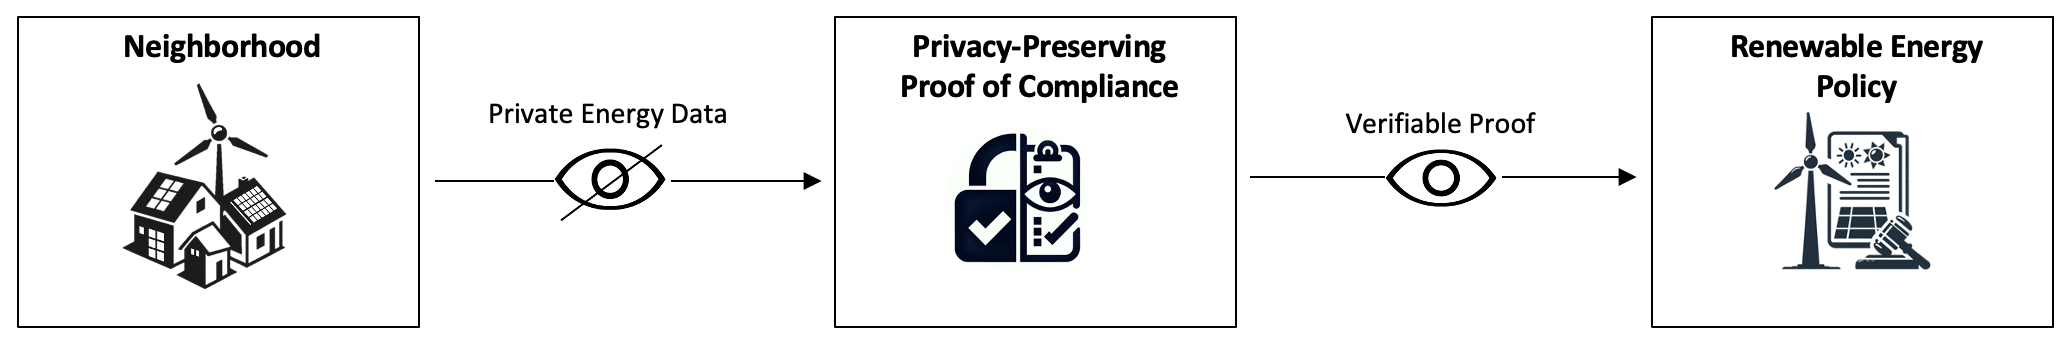
\includegraphics[width=1.5\columnwidth]{img/intro.png}
  \caption{Privacy-preserving verifiable proof of compliance for renewable energy consumption}\label{fig:intro}
\end{figure*}

	\section{Implementation}
	\label{sec:implementation}
	In this section, we describe our proof-of-concept implementation of the system proposed in Section IV. The overall architecture is depicted in Figure \ref{fig:impel}. 

\begin{figure}[H]
  \centering
  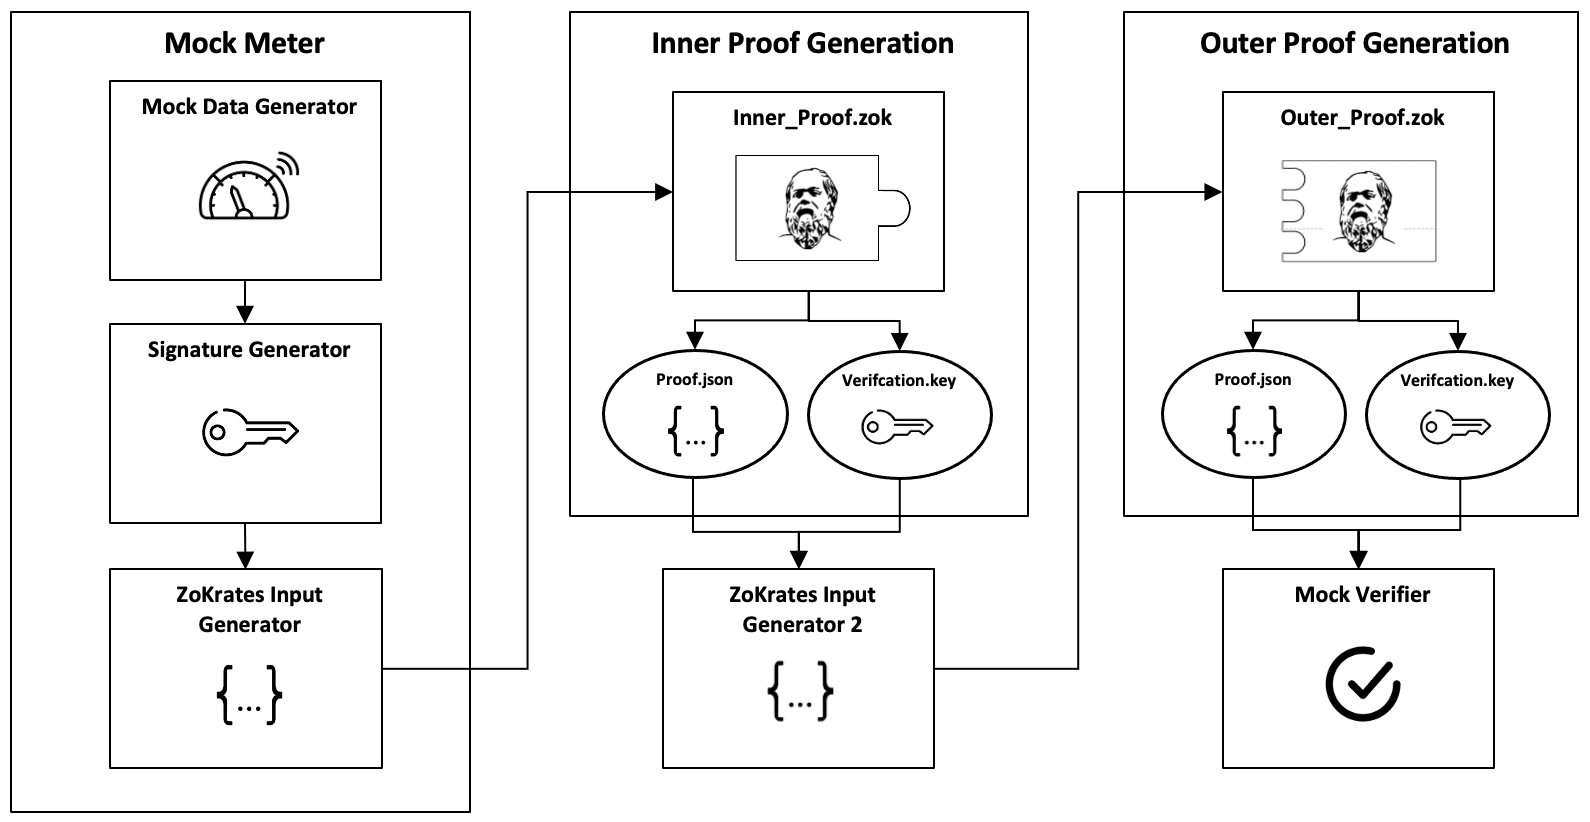
\includegraphics[width=7cm]{img/impel.png}
  \caption{Schematic illustration of the implementation's components and their interactions}
  \label{fig:impel}
\end{figure}

\subsection{Mock Meter}
Inspired by Eberthardt's et al. \cite{DecentralizedEnergyTradingMockSensor} "mock sensor for decentralized energy trading", a mock smart meter has been implemented in Python that provides energy data and generates the required input file that is utilised in the inner proof's generation. The implementation produces mocked energy data based on Gaussian regression to simulate energy data measured in kWh. Furthermore, a household internal netting or energy balance for a given interval is calculated, in order to minimise the number of variables that need to be aggregated later. 

A peculiarity is, that a specific signature is required that is compatible with the elliptic curve used in the inner proof's computation. Therefore a special implementation of the ZoKrates PyCrypto package \cite{BachelorThesisGitHub} is utilised to sign the energy readings on the decaf377 curve. 

Finally, an \texttt{inputs.json} file is created that contains all data in the correct input format for ZoKrates. 

\subsection{Inner Proof Generation}
The inner proof of integrity is computed using the mock meter's input  file. The smart meter's signature is verified and the correctness of the publicly provided net result ensured. ZoKrates' standard library does not support the for nesting required BLS12\_377 (decaf377) curve for signature verification. 
Therefore, Mehrpoya's implementation of the decaf377 curve in ZoKrates \cite{BachelorThesisGitHub} is utilised and the corresponding \texttt{verifyEddsa} function imported that allows the verification of the smart meter's signature inside the inner proof.

\subsection{ZoKrates Input Generator 2}
The input generator collects all \texttt{proof.json} files and \texttt{verification.key} files from all households and streamlines them into a suitable json format that can be utilised to compute the outer proof. 

\subsection{Outer Proof Generation}
The outer proof verifies the correctness of all inner proofs as well as the compliance of the aggregated energy balances with the threshold. As the outer proof utilises a different elliptic curve than the inner proof, negative energy balances are converted from Bls3\_77 to bw6\_761.

\subsection{Mock Verifier}

Since the nested proof compiled on the bw6\_761 curve is not verifiable on Ethereum today, a mock verifier in Python is also implemented, that verifies the proof inside a ZoKrates environment. 

	\section{Evaluation}
	\label{sec:evaluation}
	In this section the implementation of the nested proof system is evaluated. The evaluation included measuring the system’s scalability and data handling capacity. This includes measuring the maximum number of inner proofs it can support within a given compiling time and assessing the volume of energy data it can process and verify. For the sake of simplicity and demonstrability only the proof generation time is evaluated here, as  the compilation and setup only need to be executed once.
The evaluation was conducted on a consumer laptop with a 1.6 GHz Dual-Core Intel Core i5 chip. 

The inner proof’s scalability was assessed by evaluating the impact of the amount of signatures that are verified within the proof while the outer proof's scalability was asses by the amount of inner proofs that that are provided. In both cases an exponential trend can be witnessed, as can be seen in Figure \ref{figure:number_of_innner}. This exponential growth in the proof’s computation time highlights ZoKrates scalability issues. While computational performance may improve with better hardware, the clear exponential trend indicates persistent scalability limitations. Furthermore, this limits the possibility of out- sourcing larger computations of the outer proof into the inner proofs. Adding more layers of proofs to split the computational load further is currently not supported for nesting in ZoKrates, which allows scalability improvement through nesting only to a small degree of two layers.

\begin{figure}[h]
\centering
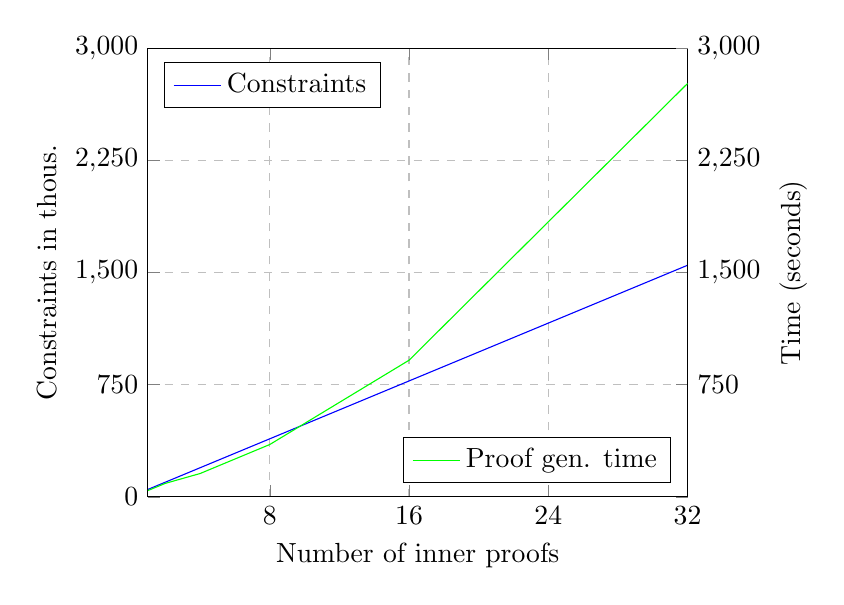
\begin{tikzpicture}
\begin{axis}[
    xlabel={Number of inner proofs},
    ylabel={Constraints in thous.},
    xmin=1, xmax=32,
    ymin=0, ymax=3000,
    xtick={8,16,24,32},
    ytick={0,750,1500,2250,3000},
    legend pos=north west,
    grid=major, % Enables major gridlines
    grid style=dashed,
]

\addplot[
    color=blue,
    mark=smooth,
    ]
    coordinates {
    (1,49.522)(2,97.912)(4,194.692)(8,388.252)(16,775.372)(32,1549.612)
    };
    \addlegendentry{Constraints}

\end{axis}

\begin{axis}[
    axis y line*=right,
    axis x line=none,
    xmin=1, xmax=32,
    ymin=0, ymax=3000,
    ylabel={Time (seconds)},
    ytick={750,1500,2250,3000},
    legend pos=south east,
]

\addplot[
    color=green,
    mark=smooth,
    ]
    coordinates {
    (1,42)(2,90)(4,156)(8,350)(16,914)(32,2766)
    };
    \addlegendentry{Proof gen. time}

\end{axis}
\end{tikzpicture}

\caption{Comparison of constraints and proof generation time for various numbers of inner proofs}
\label{figure:number_of_innner}
\end{figure}

However, as our evaluation was conducted merely up to 32 inner proofs or and signatures, we estimate the proof generation time for a higher number of inner proofs.   

Eberhardt et al. \cite{Netting} aimed for a proof generation time under 15 minutes for their netting proof with ZoKrates. However, in their system, the netting algorithm and proof generation require a more frequent execution. In contrast, the system proposed in this thesis needs to be executed less frequent. Assuming that the local utility has no hardware restrictions, unlike the smart meters or households, the proof generation time can extend multiple hours or even days. 

From 16 to 32 inner proofs, the base \( a \) of the proof generation time is 2.6 and increases for 1.16 each doubling of inner proofs, as observed from eight to 16 and 16 to 32. Assuming that the growth factor of \( a \) does not change, we can estimate the proof generation time (in seconds) for a given amount of inner proofs. We therefore modified the core formula for exponential growth , \( y = a^x \), for a scenario with a doubling of \( x \) and with a multiplicative increase of \( y \). In doing so logarithms are applied to convert the multiplicative relationships into additive ones, which can then be modelled through exponents. As the exponential growth does not start at \( x = 0 \), the formula is adjusted to account for an arbitrary starting point. Here, \( x \) represents the number of inner proofs, while \( y \) represents the proof generation time of the outer proof and \( y_0 \) represent the outer proof's generation time for the starting point \( x_0 = 32\), which is the maximum extent of my evaluation's computation.
 

\[
y = y_0 \cdot a^{\log_2\left(\frac{x}{x_0}\right)}
\]

\[
9709 = 2766 \cdot 3,51^{\log_2\left(\frac{64}{32}\right)}
\]

\[
45864 = 2766 \cdot 4,07^{\log_2\left(\frac{128}{32}\right)}
\]



With around 43 inner proofs, a proof generation time of approximately one hour is reached. The witness generation time accounts on top of that for about 10 to 20 percent of the proof generation time. Therefore, in realistic numbers, even fewer inner proofs can be nested for a computation time of one hour. Three hours of proof generation time allow for 96 inner proofs, assuming that the growth factor of \( a \) does not accelerate. Figure \ref{figure:estim} illustrates the continuation of the exponential trend for the proof generation time based on the introduced calculation.

\begin{figure}[h]
\centering
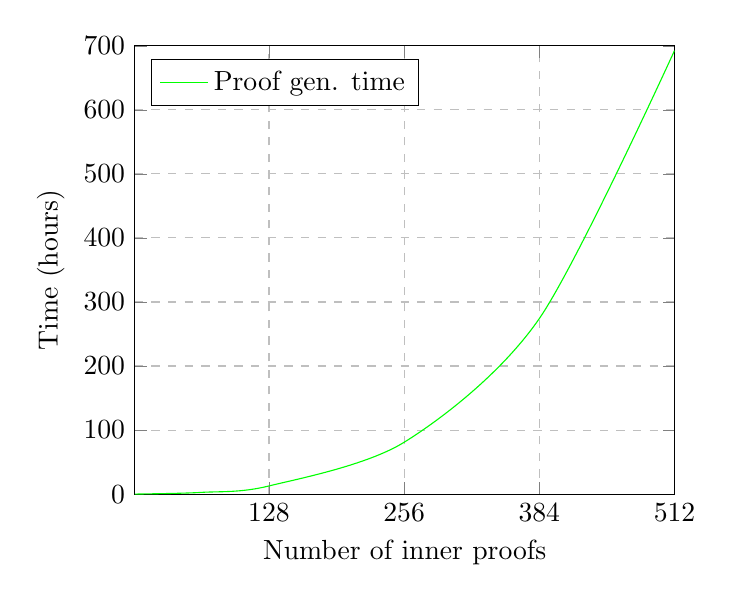
\begin{tikzpicture}
\begin{axis}[
    xlabel={Number of inner proofs},
    ylabel={Time (hours)},
    xmin=1, xmax=512,
    ymin=0, ymax=700,  % Adjusted to the max value provided in hours
    xtick={128,256,384,512},
    ytick={0,100,200,300,400,500,600,700},
    legend pos=north west,
    grid=major, % Enables major gridlines
    grid style=dashed,
]

\addplot[
    color=green,
    mark=none,
    smooth,
    ]
    coordinates {
    (1,42/3600)(2,90/3600)(64,9709/3600)(128,45864/3600)(256,291519/3600)(384,986877/3600)(512,2493276/3600)
    };
    \addlegendentry{Proof gen. time}

\end{axis}
\end{tikzpicture}

\caption{Estimating proof generation time per number of inner proofs}
\label{figure:estim}
\end{figure}


To better illustrate the requirements for a use case as presented in this paper, one district or neighbourhood within an eight-digit postal code area in Germany averages around 500 households \cite{ptvplz82210db}. The proof generation time for 512 households is approximately 29 days, assuming no other failures, such as memory constraints. Furthermore, the compiled circuit would have a size of around 264 GB and the proving key a size of around 51 GB, assuming a linear growth in those. This highlights ZoKrates scalability limits again, as such a system implemented in ZoKrates may accommodate only smaller communities and neighbourhoods.

	\section{Conclusion}
	\label{sec:conclusion}
	\input{contents/07_conclusion}


	\bibliographystyle{IEEEtran}
	\bibliography{./references}

	\vspace{12pt}

\end{document}
